\begin{figure}
    \centering
    \resizebox{0.48\textwidth}{!}{%
        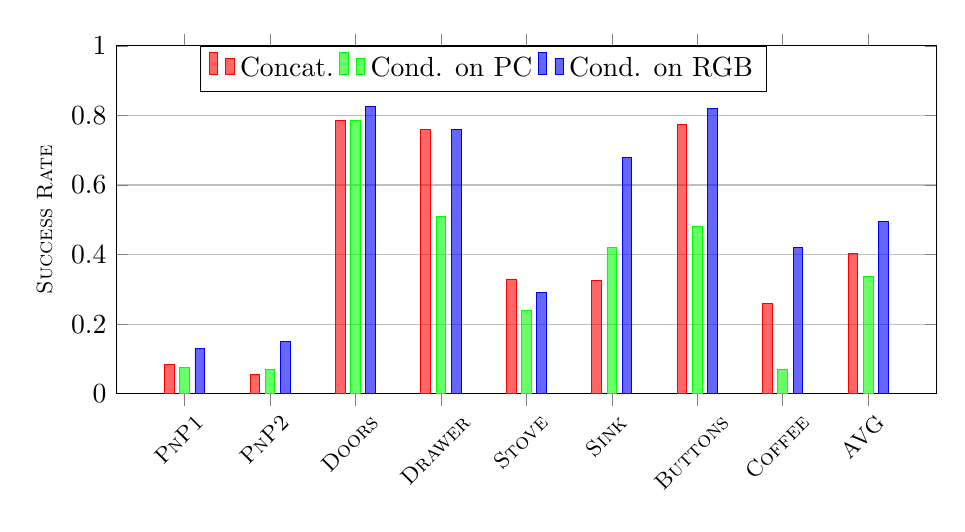
\begin{tikzpicture}[baseline]
        \definecolor{lightgray204}{RGB}{204,204,204}
        \definecolor{crimson}{RGB}{214,39,40}
        \definecolor{darkgray}{RGB}{176,176,176}
        \definecolor{darkorange}{RGB}{255,127,14}
        \definecolor{darkturquoise}{RGB}{23,190,207}
        \definecolor{forestgreen}{RGB}{44,160,44}
        \definecolor{goldenrod}{RGB}{188,189,34}
        \definecolor{gray}{RGB}{127,127,127}
        \definecolor{mediumpurple}{RGB}{148,103,189}
        \definecolor{orchid}{RGB}{227,119,194}
        \definecolor{sienna}{RGB}{140,86,75}
        \definecolor{steelblue}{RGB}{31,119,180}

        \begin{axis}[
            ybar,
            height=6cm, width=12cm,
            bar width=3.5pt,
            ylabel=Success Rate,
            ylabel style={
                font=\footnotesize\scshape
            },
            ymin=0, ymax=1,
            legend style={at={(0.448, 1)}, anchor=north, legend columns=-1},
            symbolic x coords={PnP1, PnP2, Doors, Drawer, Stove, Sink, Buttons, Coffee, AVG},
            xtick=data,
            xticklabel style={
                rotate=45,
                font=\footnotesize\scshape,
                % xshift=6pt,
                yshift=3pt,
            },
            ymajorgrids
        ]
        
        % -- First plot (Concat.) --
        \addplot [
            draw=red,
            fill=red,
            line width=.1mm,
            fill opacity=0.6
        ] coordinates {
            (PnP1, 0.0850)
            (PnP2, 0.0550)
            (Doors, 0.7850)
            (Drawer, 0.7600)
            (Stove, 0.3300)
            (Sink, 0.3267)
            (Buttons, 0.7733)
            (Coffee, 0.2600)
            (AVG, 0.4042)
        };

        % -- Second plot (Cond. on PC) --
        \addplot [
            draw=green,
            fill=green,
            line width=.1mm,
            fill opacity=0.6
        ] coordinates {
            (PnP1, 0.0750)
            (PnP2, 0.0700)
            (Doors, 0.7850)
            (Drawer, 0.5100)
            (Stove, 0.2400)
            (Sink, 0.4200)
            (Buttons, 0.4800)
            (Coffee, 0.0700)
            (AVG, 0.3358)
        };

        % -- Third plot (Cond. on RGB) --
        \addplot [
            draw=blue,
            fill=blue,
            line width=.1mm,
            fill opacity=0.6
        ] coordinates {
            (PnP1, 0.1300)
            (PnP2, 0.1500)
            (Doors, 0.8250)
            (Drawer, 0.7600)
            (Stove, 0.2900)
            (Sink, 0.6800)
            (Buttons, 0.8200)
            (Coffee, 0.4200)
            (AVG, 0.4942)
        };

        \legend{Concat., Cond. on PC, Cond. on RGB}
        \end{axis}
        \end{tikzpicture}

    }
    \caption{Success rates using different fusion types for point cloud and RGB images.}
    \label{fig:ablation_fusion}
\end{figure}
